\section{Resultados}
\begin{frame}{Resultados}
  \framesubtitle{Protótipos}
  \begin{tikzpicture}[overlay, remember picture]
    \node[anchor=center,xshift=0pt,yshift=-20pt] at (current page.center) {
      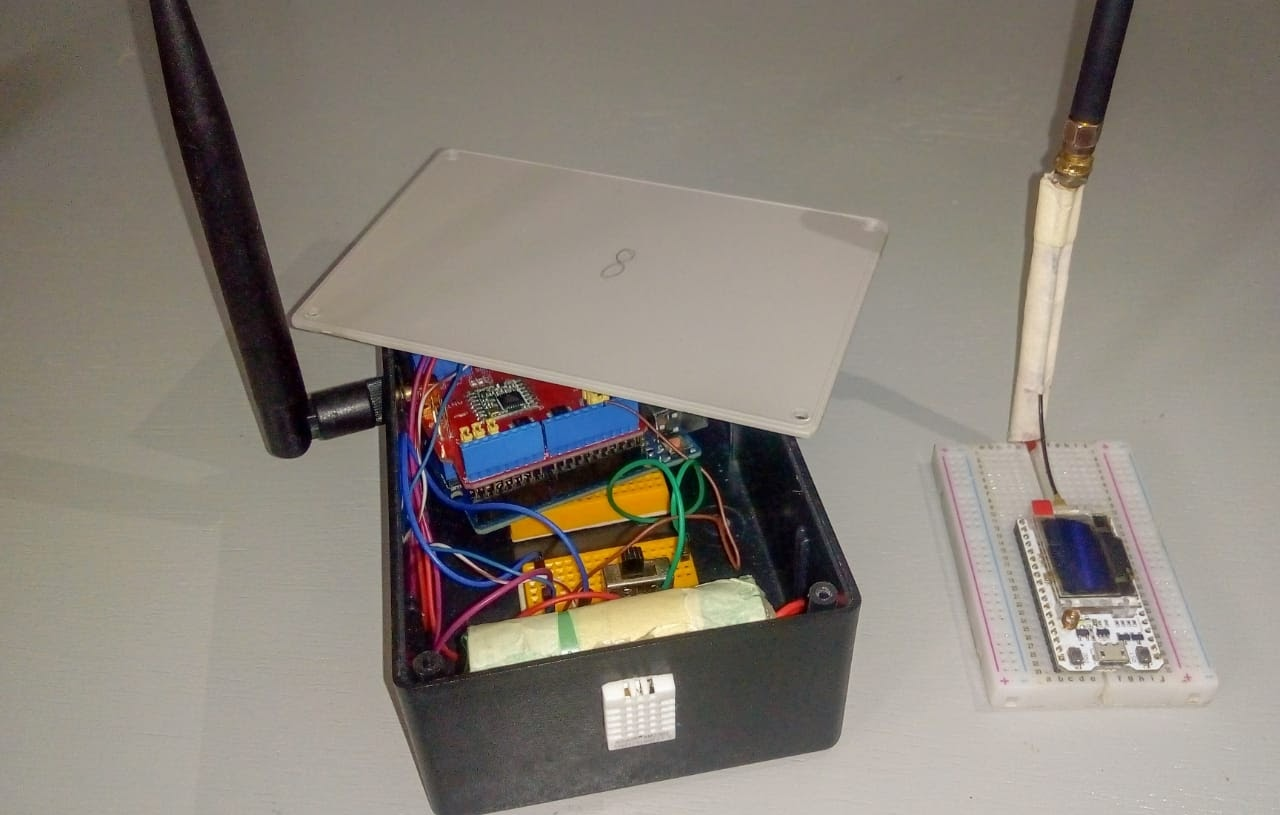
\includegraphics[height=60mm]{./assets/proto-1.jpeg}
    };
  \end{tikzpicture}
\end{frame}

\begin{frame}{Resultados}
  \framesubtitle{Protótipos}
  \begin{tikzpicture}[overlay, remember picture]
    \node[anchor=center,xshift=0pt,yshift=-20pt] at (current page.center) {
      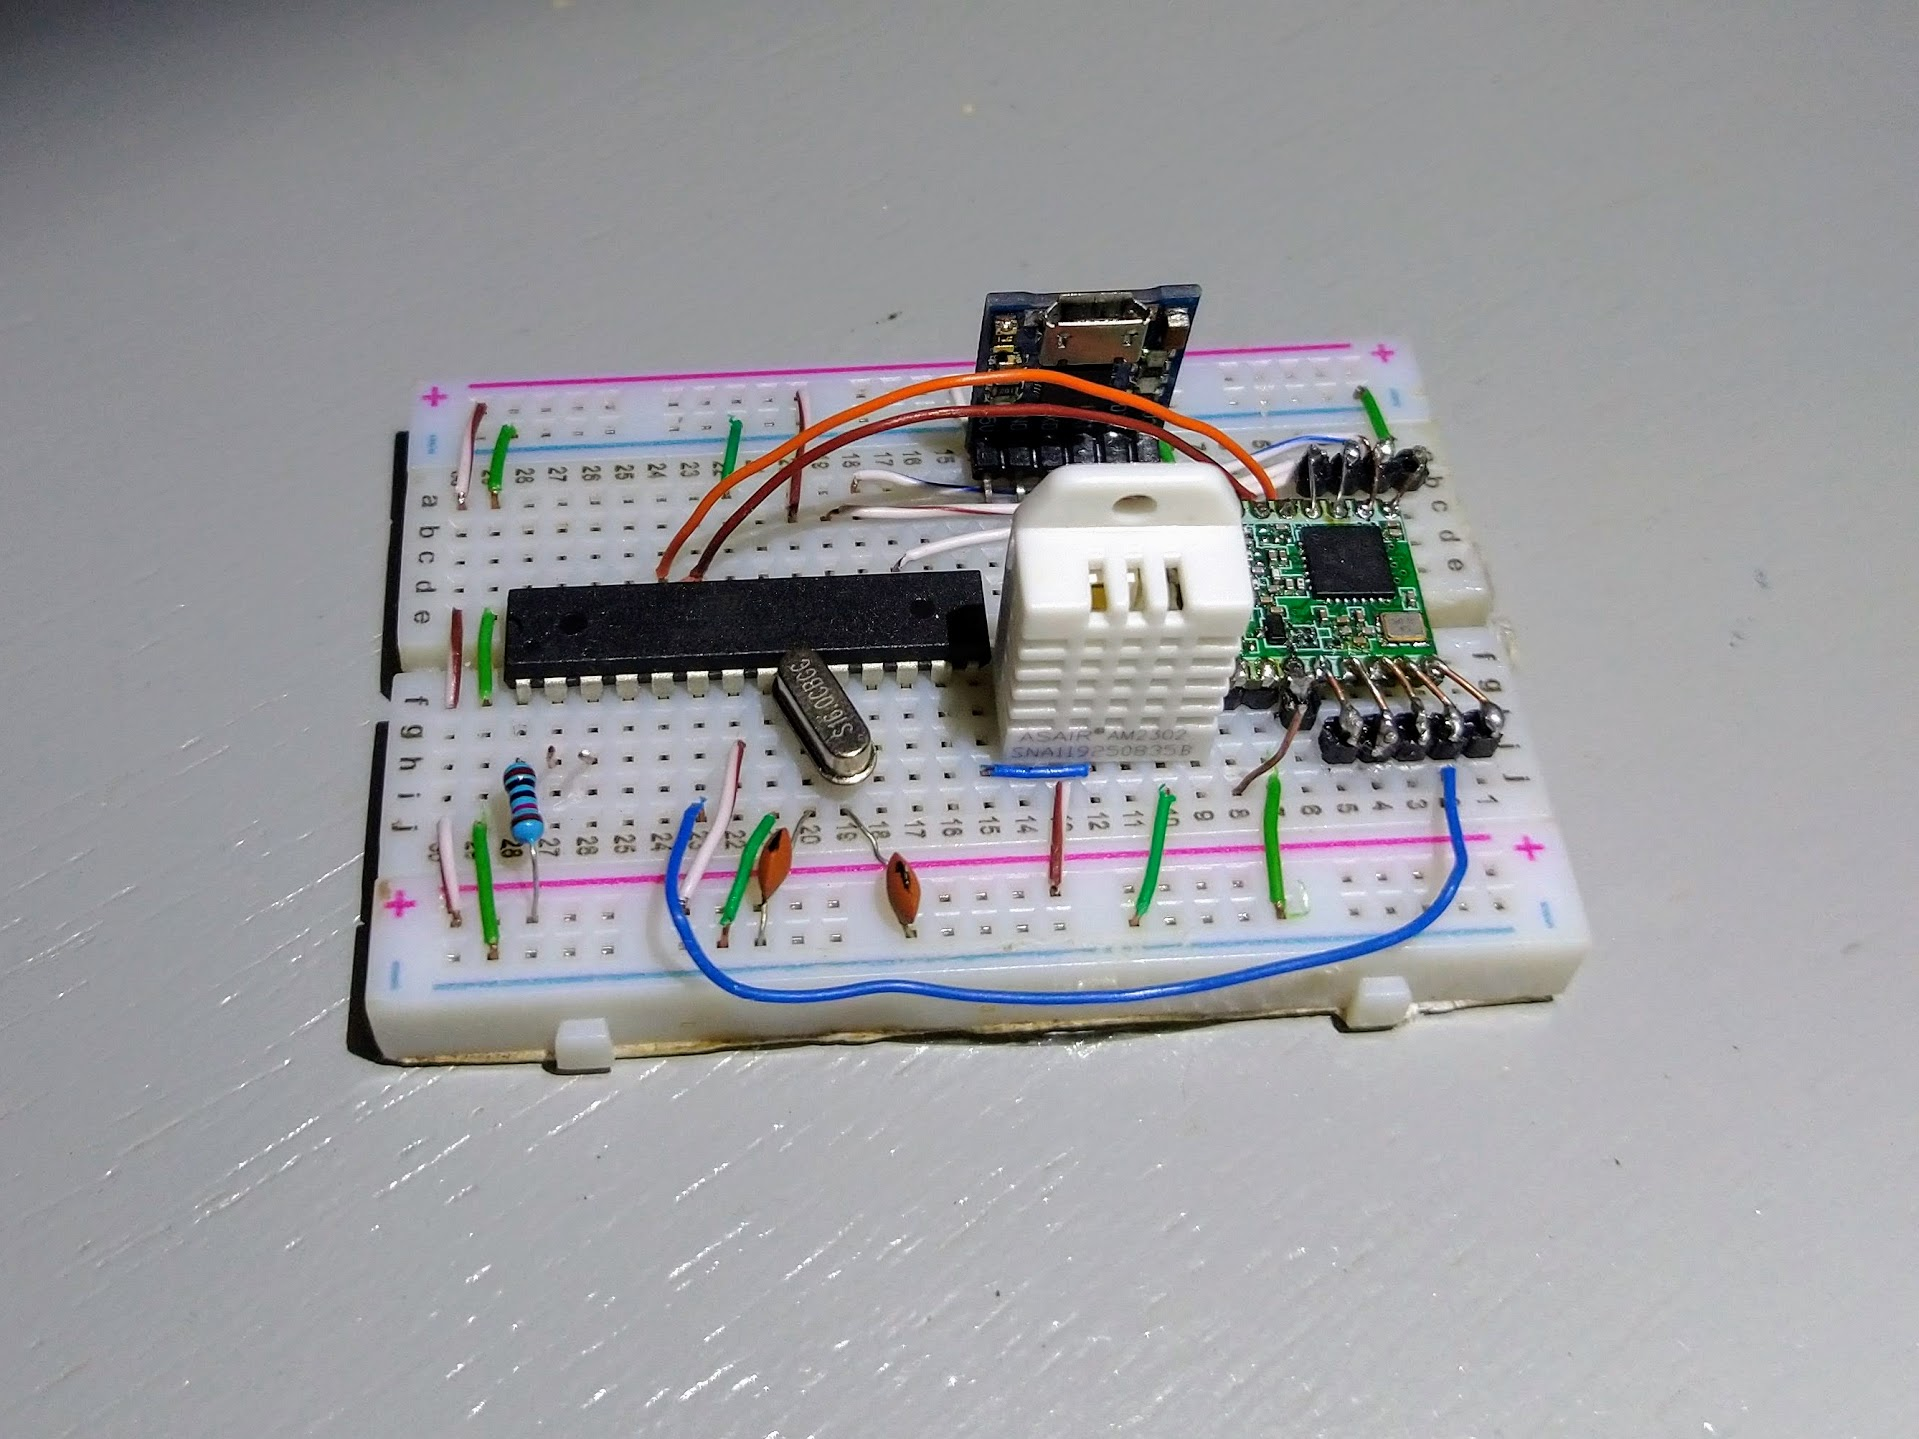
\includegraphics[height=60mm]{../assets/end-node-proto-2.png}
    };
  \end{tikzpicture}
\end{frame}

\begin{frame}{Resultados}
  \framesubtitle{Metodologia dos testes}
  \begin{itemize}
    \item Verificar a viabilidade da aplicação
    \begin{itemize}
      \item Transmissão entre os dispositivos
      \item Consumo energético
      \item Custo de produção
    \end{itemize}
  \end{itemize}
\end{frame}

\begin{frame}{Análise de Transmissão dos Pacotes}
  \framesubtitle{Ambiente}
  \begin{itemize}
    \item Bloco dos Professores
    \item Entre o Lab. Assert e o Lab. GComPI
    \item Distância de 60 metros para testes
  \end{itemize}
  \begin{tikzpicture}[overlay, remember picture]
    \node[anchor=south,xshift=0pt,yshift=35pt] at (current page.south) {
      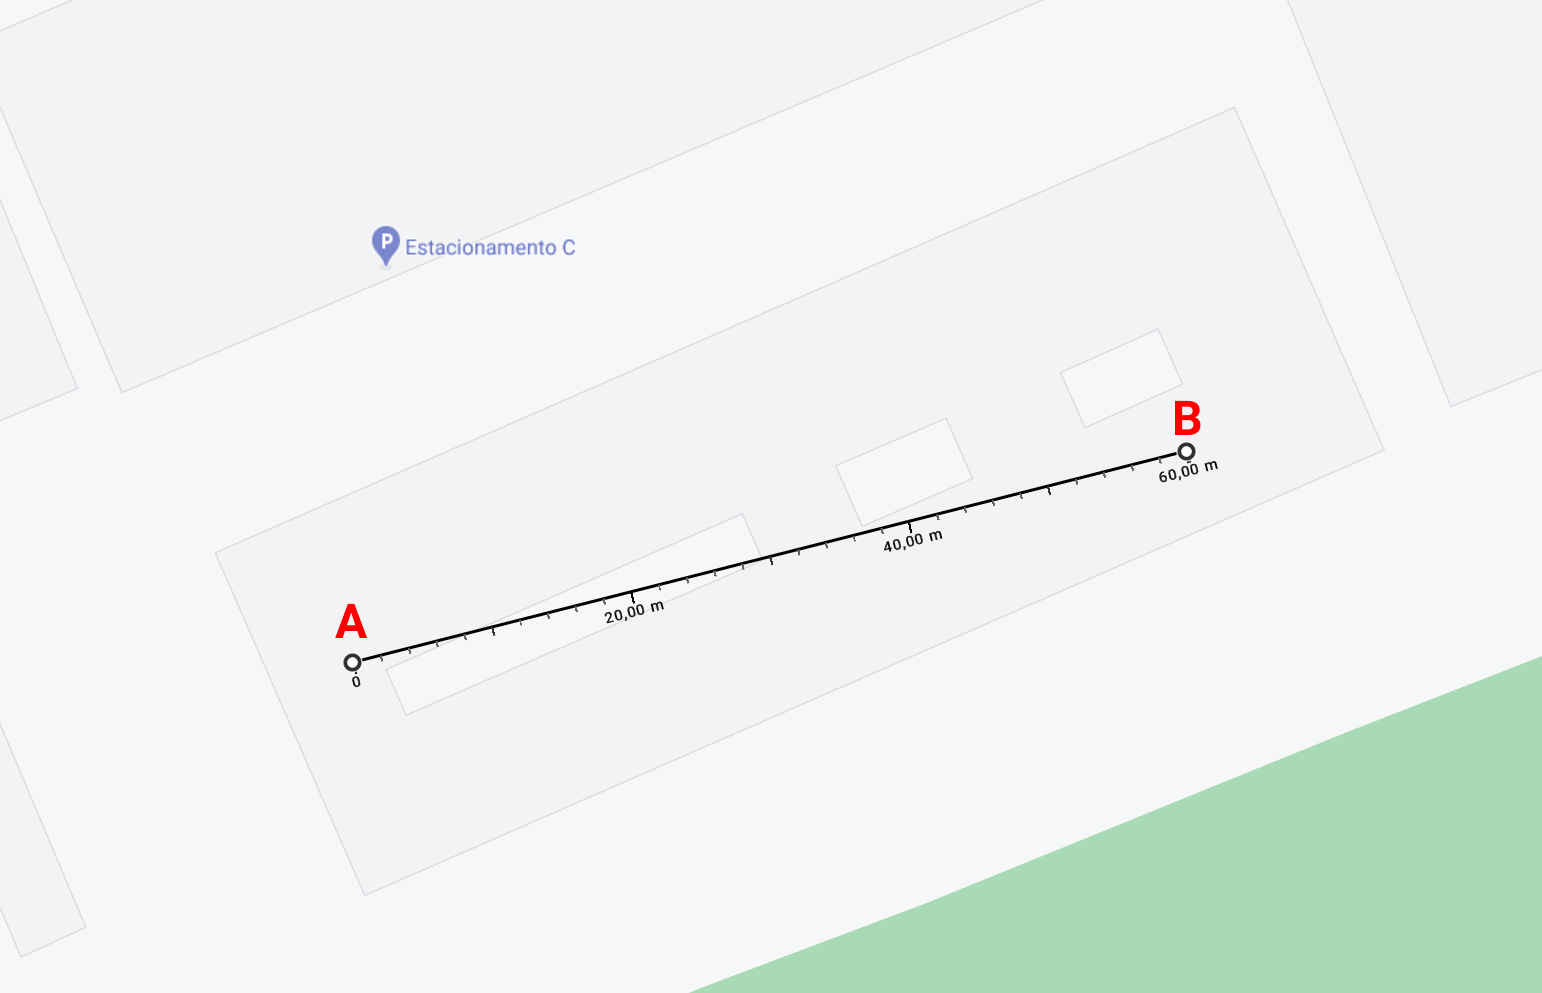
\includegraphics[height=35mm]{../assets/experiment-01.png}
    };
  \end{tikzpicture}
\end{frame}

\begin{frame}{Análise de Transmissão dos Pacotes}
  \framesubtitle{Teste}
  \begin{itemize}
    \item Dispositivos ligados na tomada
    \item Transmitindo 1 pacote a cada 5 minutos
    \item Duração de 5 dias
    \item Servidor na Microsoft Azure
  \end{itemize}
\end{frame}

\begin{frame}{Análise de Transmissão dos Pacotes}
  \framesubtitle{Dia 21 de abril de 2020}
  \begin{tikzpicture}[overlay, remember picture]
    \node[anchor=center,xshift=0pt,yshift=-15pt] at (current page.center) {
      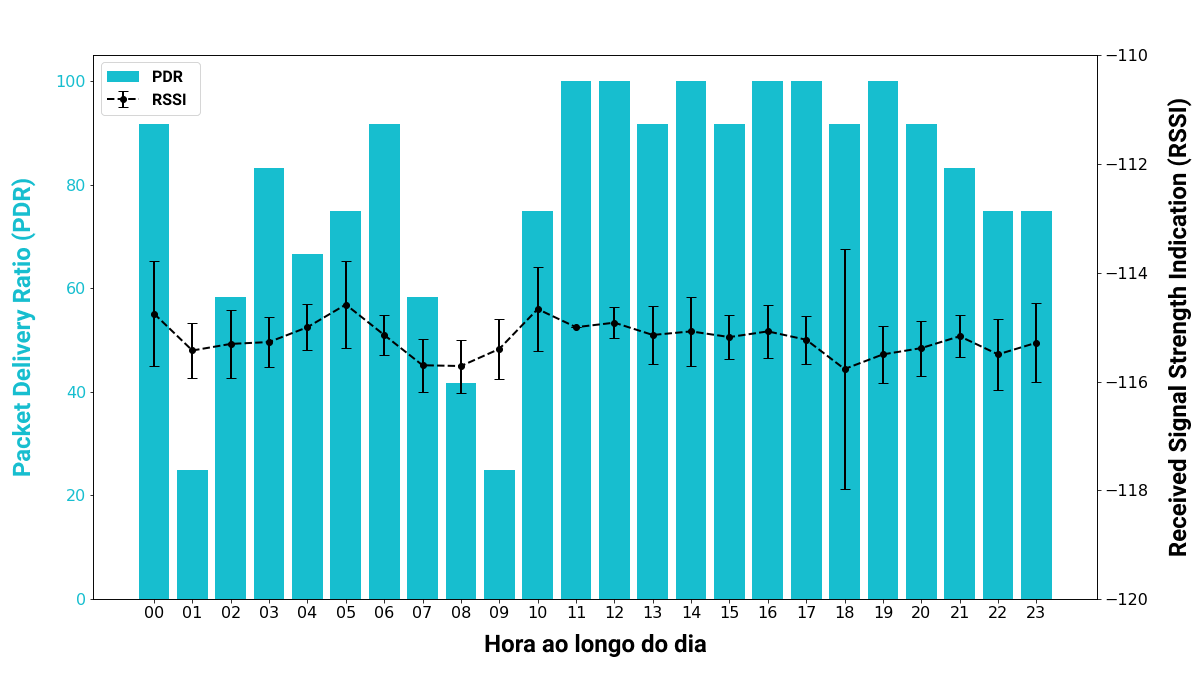
\includegraphics[height=50mm]{../assets/21-04-2020-pdr-rssi.png}
    };
  \end{tikzpicture}
\end{frame}

\begin{frame}{Análise do Consumo Energético}
  \framesubtitle{Passos para calcular a duração da bateria}
  \begin{itemize}
    \item Realizar as medições nos diversos pontos do dispositivo
    \item Calcular a média do consumo de acordo com as medidas coletadas
    \item Dividir a capacidade da bateria pelo consumo médio do dispositivo
  \end{itemize}
\end{frame}

\begin{frame}{Análise do Consumo Energético}
  \framesubtitle{Teste para cada protótipo}
  Primeiro protótipo
  \begin{itemize}
    \item Teste realizado em dezembro de 2019
    \item Medições realizadas utilizando um osciloscópio
    \item Auxílio de um resistor de derivação e um amplificador
  \end{itemize}

  \bigskip Segundo protótipo
  \begin{itemize}
    \item Teste realizado em março de 2021
    \item Teste teórico devido a dificuldade do acesso ao equipamento
    \item Dados retirados dos \textit{datasheets} dos componentes
  \end{itemize}
\end{frame}

\begin{frame}{Análise do Consumo Energético}
  \framesubtitle{Teste para cada protótipo}
  \begin{tikzpicture}[overlay, remember picture]
    \node[anchor=center,xshift=0pt,yshift=-20pt] at (current page.center) {
      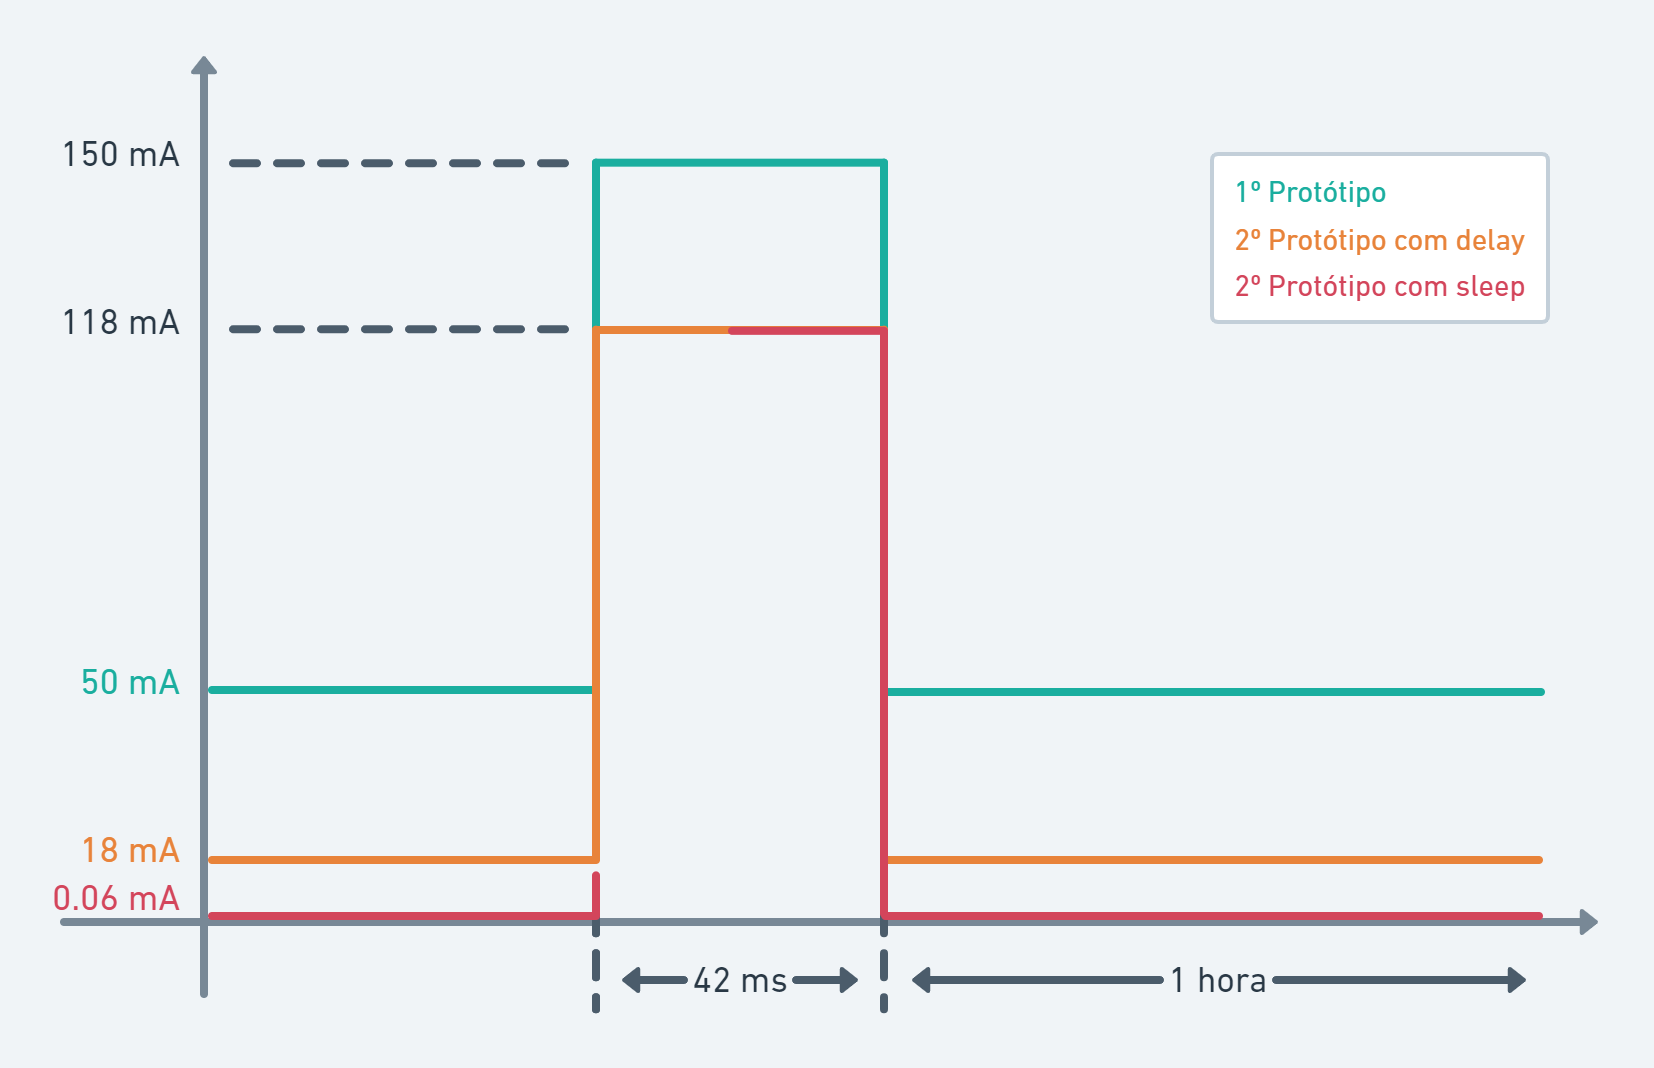
\includegraphics[height=60mm]{./assets/chart.png}
    };
  \end{tikzpicture}
\end{frame}

\begin{frame}{Análise do Consumo Energético}
  \framesubtitle{Duração da bateria nos protótipos}
  \begin{itemize}
    \item 1º protótipo: \alert{39,3 horas}
    \item 2º protótipo: \alert{122,2 horas}
    \item 2º protótipo em modo sleep: \alert{35.849 horas}
  \end{itemize}
\end{frame}

\begin{frame}{Análise do Custo de Produção}
  \framesubtitle{\textcolor{fibeamer@black}{Geral}}
  \begin{table}[!b]{
    \scalebox{0.9} {
      \carlitoTLF % Use monospaced lining figures
      \begin{tabularx}{\textwidth}{lrr}
        \textbf{Componente}&\textbf{Preço no Brasil}&\textbf{Preço na China}\\
        \toprule
        1x ATmega328 & R\$ 19,90 & R\$ 09,12 \\
        1x LoRa RFM95W 915Mhz & R\$ 56,00 & R\$ 20,99 \\
        1x Bateria 18650 3000mAh & R\$ 19,90 & R\$ 17,65 \\
        1x Cristal Oscilador 16mhz & R\$ 01,47 & R\$ 00,46 \\
        1x Capacitor de cerâmica 100pF & R\$ 00,05 & R\$ 00,04 \\
        2x Capacitor de cerâmica 22pF & R\$ 00,22 & R\$ 00,08 \\
        2x Resistores de 10k Ohms & R\$ 00,12 & R\$ 00,06 \\
        \bottomrule
        \textnormal{\alert{Total}} & \alert{R\$ 97,66} & \alert{R\$ 48,40}
      \end{tabularx}
    }
  }
    \caption{Custos referente as peças do segundo protótipo.}
  \end{table}
\end{frame}